\begin{figure}
    \centering
    \setlength{\resLen}{0.8in}
    \setlength{\raiseLen}{0.9in}
    \addtolength{\tabcolsep}{-3.5pt}
    \small
    %
    \begin{tabular}{cccc}
        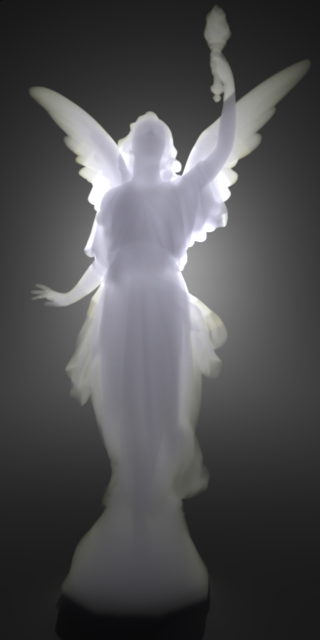
\includegraphics[width=\resLen]{images/lucy/color.jpg} &
        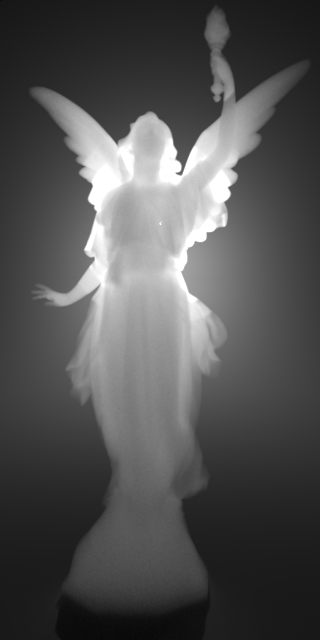
\includegraphics[width=\resLen]{images/lucy/color_400nm.jpg} &
        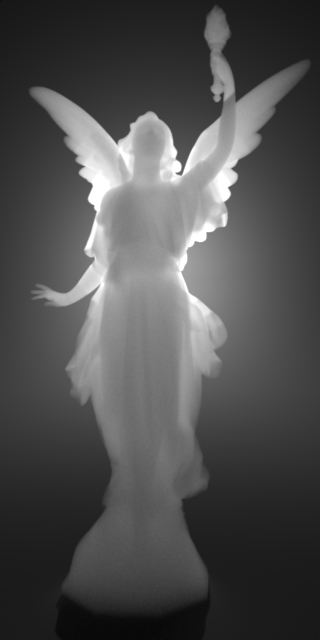
\includegraphics[width=\resLen]{images/lucy/color_550nm.jpg} &
        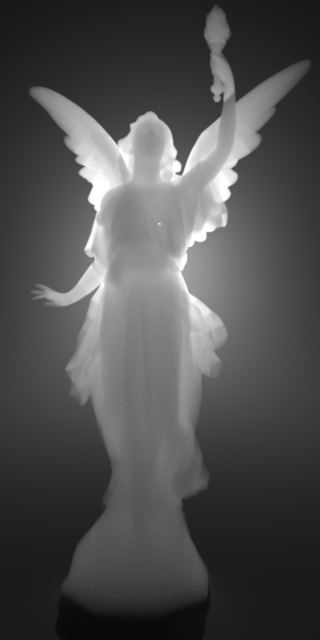
\includegraphics[width=\resLen]{images/lucy/color_700nm.jpg}
        \\
        \textbf{(a) Multi.} & \textbf{(b) 400nm} & \textbf{(c) 550nm} & \textbf{(d) 700nm}
    \end{tabular}
    \caption{\label{fig:multiwave2}
        (a)~Multi-spectral rendering of a homogeneous Lucy model using identical bulk scattering parameters as the top row of Figure~\ref{fig:multiwave1}.
        (b--d)~Monochrome renderings of the same model at three wavelengths.
    }
\end{figure}

% \raisebox{\raiseLen}{\multirow{2}{*}{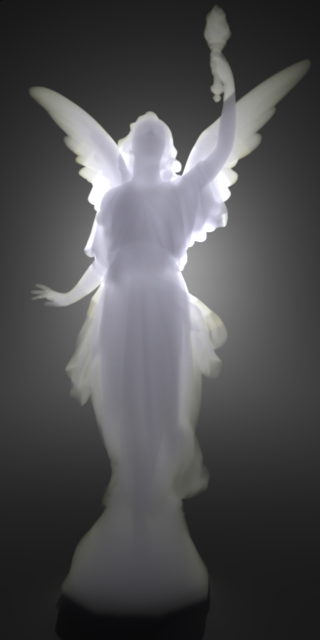
\includegraphics[width=\resLen]{images/lucy/color.jpg}}} & 
\includegraphics[width=\resLen]{images/placeholder3.jpg} \\
% & 
\includegraphics[width=\resLen]{images/placeholder3.jpg}
